\chapter{Data Distribution Service}
\section{Overview}
The concept of distributed applications is to enable seamless communication between systems. There are a number of different ways to achieve this and the one we are focusing on is Data distribution service for real-time systems (DDS).
It is a standard developed by Object Management Group (OMG) that enables communication between computers, that is decoupled in space, time and flow. This means that the computers don't have to know each other and they don't have to be ready to receive when a message is sent. It uses a publish/subscribe pattern to send and receive messages that can be customised by a list of quality of service parameters.

\section{Middleware}

\subsection{What and why?}
To achieve this seamless communication some layer of software is needed to handle the network communication and distribution of data. This layer of software is called middleware.

Middleware can be defined by this quote:

"A layer of software residing on every machine, sitting between the
underlying operating system and the distributed applications,
whose purpose is to mask the heterogeneity of the cooperating
platforms and provide a simple, consistent and integrated
distributed programming environment."\footnote{Coulouris, G., J. Dollimore, T. Kindberg, and G. Blair (2001). Distributed systems: Concepts and design. Pearson.}

DDS implements the Publish/Subscribe middleware paradigm that is described in the next section.

\subsection{Alternatives to DDS}



There are a number of different implementations of middleware in distributed systems where Publish/Subscribe as used in DDS is just one example. An alternative is Enterprise Messaging System (EMS) that is a set of standards that allows organisations to send messages between computer systems using standard formats like XML and SOAP.
TIBCO Enterprise Messaging Service is an example of implementation of EMS.

TIBCO EMS could be used as a real time messaging system in a big cooperation. It is secure as it uses TSL/SSL, it is reliable and scalable via load balancing and guaranteed message delivery models. And it supports a wide array of technologies that secures easy development and reuse of existing systems.

\section{Publish/Subscribe pattern}
The publish/subscribe pattern is a well known programming paradigm. It is more well known in the form of the Observer Pattern described by Gang of Four \footnote{\citep{DesignPatterns}}
The idea of the publish/subscribe pattern is loosening the coupling between a publisher and a subscriber. A publisher is a entity that has some data or content to deliver or distribute. A subscriber is interested in obtaining this information when it is published, but without needing to know where it is published from.
The subscriber subscribes to a topic or type at a EventService of some kind. When a publisher notifies the EventService with the new data, The EventService will notify the concerned subscribers. This is illustrated in the figure below.

\begin{center}
	\fbox {
	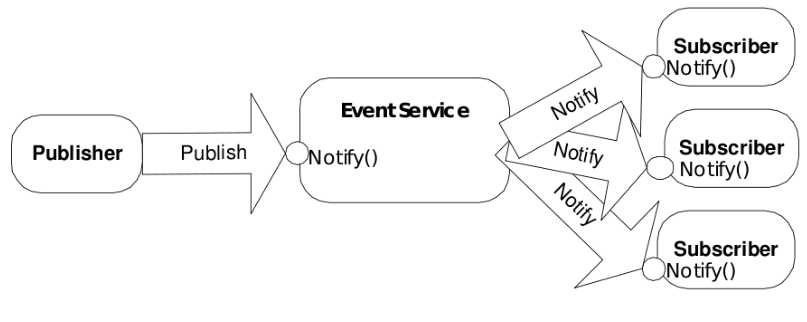
\includegraphics[width=\textwidth]{PublishSubscribe_Pattern.png}
	}
	\captionof{figure}{Sublish/Subscribe pattern from 02_DDS slideshow}
\end{center}

This is the same approach used by DDS. The Middleware must act as the EventService, and the 

\subsection{Coupling}


\subsection{Topic based}
\subsection{Content based}
\subsection{Type based}


\section{Real-time systems}


\section{Quality Of Service}
For setting up the connections between entities, Publishers, Middleware and Subscribers must agree on certain terms. Quality of Service (QoS) lets the middleware know how to treat connections between publishers and subscribers as well as how to treat messages.

The QoS lets us setup \textit{terms} of the communication. This can be used, for instance, to set up the \textit{lifetime} of a message. This way, we could make sure a message will stop being interesting to subscribers after a while. 

Another example is setting the \textit{deadline} parameter on a subscribers QoS. This tells publishers, that the subscriber expects data within the specified timeframe. This way, if the middleware detects a QoS of the publisher, which will transfer data at a slower rate than what the subscriber requests, the middleware will \textbf{not} connect these two.

The QoS can be set programmatically through properties and structs in the respective classes or through XML configuration files. 


\section{Connext RTI}


\subsection{Configuration on linux}